\chapter*{Introduzione}
Negli ultimi anni, grazie all'avvanto di nuove tecnologie nel settore delle reti wireless
e dei dispositivi mobili le reti wireless sono diventate una parte fondamentale
dell'infrastruttura delle telecomunicazioni. Oramai l'utente pretende che la qualita
delle reti wirless siano almeno pari a quelli forniti via cavo visti gli incredibili passi avanti
che le reti cellulare hanno ottenuto negli ultimi 5-6 anni.
Basti pensate alla nuove reti 4G (LTE e WiMax) che promettono velocita nell'ordine sui 5-8 Mbps
di Mbit/s in download e contro le attuali linea ADSL con una media di 15 Mbps promessi.
In piu le attuali societa telefoniche foniscono piu facilemente reti wireless ad alta velocita
piuttosto che reti cablate visto la diffusione di apparecchiature mobile quali smartphone, tablet, ecc [Vedi Figura 1].
\begin{figure}
\begin{center}
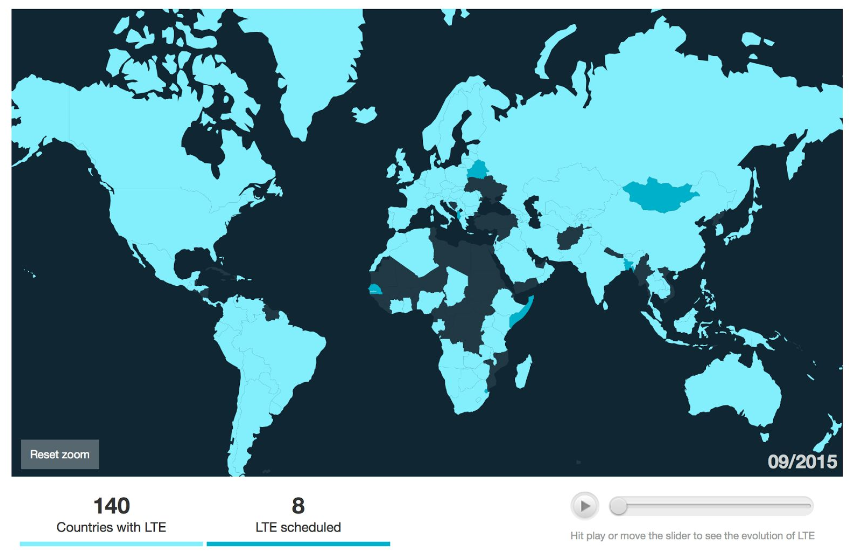
\includegraphics[scale=0.5]{LTE_Country_09_2015.png}
\caption[Cop LTE]{Copertura LTE mondiale}
\label{etichetta}
\end{center}
\end{figure}
In piu con gli attuale progetti di Facebook e Google sulla progettazione di droni capaci di portare
reti WiFi o LTE si punta ad avere una copertura quasi totale del suolo mondiale.\\
Questa sempre piu crescente utenza connessa in movimento ha fatto acrescere l'interesse
acquisire informazioni contestuali per poter offrire servizi di maggior interesse e utilita
per l'utente. L'informazione contestuale puo riferirsi alla posizione dell'utente, all'ora attuale,
a proprieta fisiche come la temperatura, ecc.
La gestione efficiente del contesto richiede un dettagliato data modeling ottenuto
con processi specifici di classificazione, inferenza e predizione.\\
Certo e difficilmente comprendere cosa puo essere considerato context aware,
senza prima avere dato una definizione di contesto. La principale definizione
di contesto e la seguente:
\textit{Il contesto e qualsiasi informazione che puo essere usata per caratterizzare
la situazione di una entita. Una entita e una persona, un luogo ad un oggetto considerata rilevante all interazione fra l utente
e l applicativo, inclusi l utente e l applicativo stessi}
\cite{cit_48}. Il contesto dunque e specificato
mediante i valori di opportuni parametri, rappresentanti l'attivita di un'entita
L'approccio orientato al contesto quindi permette all'entita di adattarsi all'ambiente,
offrendo superiori vantaggi e possibilita ai nuovi applicativi.\\
Una delle proprieta che maggiormente si desidera nel mobile context-awareness
e la loro possibilita di poter effettuare previsioni, caratteristica che permetterebbe
lo sviluppo di nuove, avanzate applicazioni.\\
Nel 2001, il Computer Science and Telecommunications Board (CSTB) del
Consiglio Nazionale della Ricerca degli Stati Uniti d'America ha riunito una
commissione di esperti per eseguire una ricerca sulle opportunita certe e sui
possibili sviluppi relativi all'interazione tra le comunita di ricerca geo-spaziale
ed informatica. Nella relazione prodotta dalla commissione \cite{cit_47}, si evidenzia
come l'ubicazione dell'utente sia uno dei fattori fondamentali nelle diverse
definizioni di contesto che sono state proposte in letteratura. La centralita
di tale componente e la possibilita, fornita dalle attuali tecnologie mobili, di
rilevare in modo sufficientemente preciso, semplice e continuativo, la posizione
geografica degli utenti, fanno di questo settore un campo di ricerca attualmente
molto attivo.\\
Contemporaneamente alla nascita dei servizi context aware, e dunque nata
la necessita di avviare una ricerca mirata al miglioramento delle prestazioni
nella previsione delle traiettorie. Tale ramo di ricerca ovviamente mutua gran
parte della natura delle applicazioni context aware. In questo caso pero le
informazioni memorizzate si riducono a semplici dati spaziali e temporali, che
dunque non rischiano di ledere la privacy della persona come invece possono
essere portati a fare con applicativi context aware, che per loro natura cercano
di tracciare tutti gli aspetti (gusti, personalita) dell'utenza. La conoscenza della
posizione di oggetti mobili ha dunque condotto allo sviluppo di applicazioni
e servizi che sono stati catalogati location-based, che necessitano di conoscere
la posizione approssimata di un oggetto mobile per operare. Esempio di tali
servizi sono gli applicativi di navigazione, gestori di traffico e la pubblicita
location-based. In uno scenario tipico, il dispositivo mobile che sta fornendo
un determinato servizio, periodicamente informa il framework di posizionamento
della attuale posizione.\\
Nell'ultimo decennio anche i sistemi di sistemi di posizionamento sono migliorati.
da un'accuratezza di decine di metri, si e ormai arrivari ad avere una precisione
di pochi metri anche per utilizzi civili. La ricerca di una precisione sempre
piu alta a disposizione di tutti ha portato alla creazione di sistemi si posizionamento
alternativi la GPS quali GLONASS (Militare russo), COMPASS (Cina), Galileo (Europa) e IRNSS (India)
stanno cercando di imporsi come alternativa al sistema Americano.\\
Grazie alla copertura sempre crescente di reti wireless e sistemi di posizionamente la
context aware non e piu incentrata sulla ricerca della possizione attuale dell'utente, ma sulle possibili destinazioni
e percorsi nel breve e lungo termine. Grazie ad una metodologia si cerca di predire la posizione
per anticipare i movimenti dell'utente e quindi cercare di eseguire un pre-fetch
del servizio sulla localita prevista.
Lo sviluppo di pratiche ed accurate tecniche di previsione degli spostamenti
puo dunque aprire le porte a molti applicativi quali prenotazione di risorse,
servizi location-based, ma anche migliorare la pianificazione e gestione delle
aree urbane, grazie ad una migliore analisi del flusso urbano.\\
Ovviamente la possibilita di tracciare la posizione attuale dell'utente da sola non e sufficiente
ad effettuare previsioni sul futuro dell'utente. In un articolo pubblicato qualche anno fa
 \cite{new_1}, nel quale si afferma come osservando i dati storici relativi ai movimenti di un utente
(collezionati con diverse tecniche, nel caso citato accedendo alle basi di dati di una compagnia telefonica)
sia possibile individuare pattern di movimento, ed prevedere correttamente il luogo in cui
si trova una persona per il 93\% del tempo. Da tali studi emerge come ciascun
individuo abbia un insieme di localita che raramente lascia, e nelle quali si
sposta con grande regolarita. Gli utenti che risiedono stabilmente in un raggio
di 6 miglia hanno un tasso di predicibilita della posizione che va dal 93\% al
97\%, ma anche nel caso in cui il raggio aumenti di centinaia di miglia, la
percentuale delle previsioni rimane alta, stabilizzandosi al 93\% di successo.
In tale articolo vengono inoltre indicati dei legami tra le localita frequentate
dall'individuo e le ore della giornata. In particolare si evince come in
certi orari di transizione (prima o dopo l'orario di lavoro, oppure durante le
pause pranzo) le previsioni sul luogo in cui si trova l'utente vedano un brusco
peggioramento dei risultati; comunque la percentuale che l'utente si trovi in
un qualsiasi momento della giornata nella localita piu visitata e molto alta (del
70\%).

\section{Obiettivi della tesi}
Gia in precedenti lavori di tesi svoltesi nell Universita degli Studi di Udine e
stato presentato un algoritmo di previsione delle traiettorie basato sul modello
della fisica dei campi elettrici, dove le localita maggiormente importanti
per l'individuo erano caratterizzate da forze attrattive e le meno importanti
da forze nulle se non addirittura repulsive. Tale algoritmo e denominato
ARDA, e stato presentato unitamente ad una nuova proposta di pesatura dell'importanza
delle localita che prende il nome di SpaceRank, il quale andava
ad affiancare altri indici di valutazione delle localita quali TotalTime (il tempo
totale che l'individuo passa in una localita), AverageTime (il tempo medio che
l'individuo passa in una certa localita durante una visita), NumberOfVisits (il
numero di volte che l'utente passa per una certa localita), e combinazioni di
tali indici.
Il lavoro svolto in una precedente tesi \cite{new_1} proponeva:
\begin{itemize}
\item l'implementare dell'algoritmo di previsione ARDA utilizzando vari indici di valutazione
dell'importanza delle localita, con diverse suddivisioni di territorio

\item confronto dei risultati di previsione ottenuti evidenziando il comportamento
dell'algoritmo ARDA rispetto a due altri algoritmi di previsione( il primo
che suppone l'utente prosegua la propria corsa in linea retta mantenendo la
velocita media, il secondo che suppone l'utente prosegua il proprio percorso
rimanendo in un intorno del punto rilevato);

\item valutando la stabilita degli algoritmi proposti esegundo dei test anche su una diversa raccolta di punti GPS (messa a disposizione
dal Prof. Thad Starner) riguardante un territorio di dimensioni e varieta di movimenti maggiori;

\item analisi del comportamento dell'algoritmo nelle previsioni delle destinazioni finali, eseguite
lungo quattro milestone virtuali poste lungo i percorsi (inizio, 25\%, 50\% e 75\% del tracciato).

\end{itemize}

Questa tesi prende in esame l'algoritmo e i dati di quella precedentemente descritta e si pone i seguenti obbiettivi:
\begin{itemize}
\item Traduzione degli algoritmi dal linguaggio Python a Java e migliorarne alcuni aspetti;
\item Unificare le procedure di test per i vari indici;
\item Sviluppo di un'interfaccia per l'utilizzo al di fuori della riga di comando;
\item Sviluppo di un sistema di visualizzazione ed esportazione dei test eseguiti.
\end{itemize}

\section{Struttura della tesi}
Lo scritto della tesi si divide in quattro principali parti.
Nella prima parte si occupa di presentare gli algoritmi presi in esame cercando di metterne in evidenza
non solo gli aspetti modellistici, ma anche i problemi implementativi.
Nella seconda parte si da ampio spazio ai risultati ottenuti sia nei risultati che a livelli
prestazionali.
Infine la terza parte e quella conclusiva, in cui si riassume il lavoro svolto traendo
le somme sul lavoro svolto, presentando i punti di forza e di debolezza delle soluzioni
adottante dando anche dei gli spunti di riflessione su eventuali sviluppi.\\

Le tre parti sopra esposte in realta sono state svolte con diversa estensione,
cercando di rispettare le gerarchie logiche.
La prima sezione e racchiusa nel Capitolo 1 e 2.
Il primo capitolo espone i concetti e la teoria sugli algoritmi scelti, vista l'importanza di
riuscire a proporre nel modo piu esauriente possibile le soluzioni algoritmiche
adottate. Il seconto capitolo invece si sofferma sulle scelte di sviluppo fatte, gli accorgimenti fatti per migliorare
gli algoritmi e il funzionamento del programma.
La seconda parte invece si sviluppa nei segunati due capitoli.Il Capitolo 3 e 4.
Nel terzo capitolo si espongono i risultati ottenuti comparandoli con quelli
ottenuti nella tesi precedente lasciando spazio a grafici e comparative cercando
di capire il perche delle differenze.
Nel quanto capitolo si fa una piccola osservazione sulle prestazioni delle 2 versioni
facendo anche una comparativa con i tempi stimati al tempo della tesi originale.
Infine la quarta parte, quella conclusiva, nella quale si cerca con il quinto capitolo
di riassumere il lavoro svolto, evidenziando i risultati ottenuti e cercando
di proporre come poter ulteriormente sviluppare la ricerca e miglioramenti prestazionali.
